\section{Shift register con D-latch}
Si è montato uno shift register a 4 bit utilizzando 2 integrati 74LS74 che contengono 2 FF D-Latch ciascuno come in \fig{shift}. Le resistenze utilizzate sono da \SI{330}{\ohm}.

	\begin{figure}[H]
		\centering
		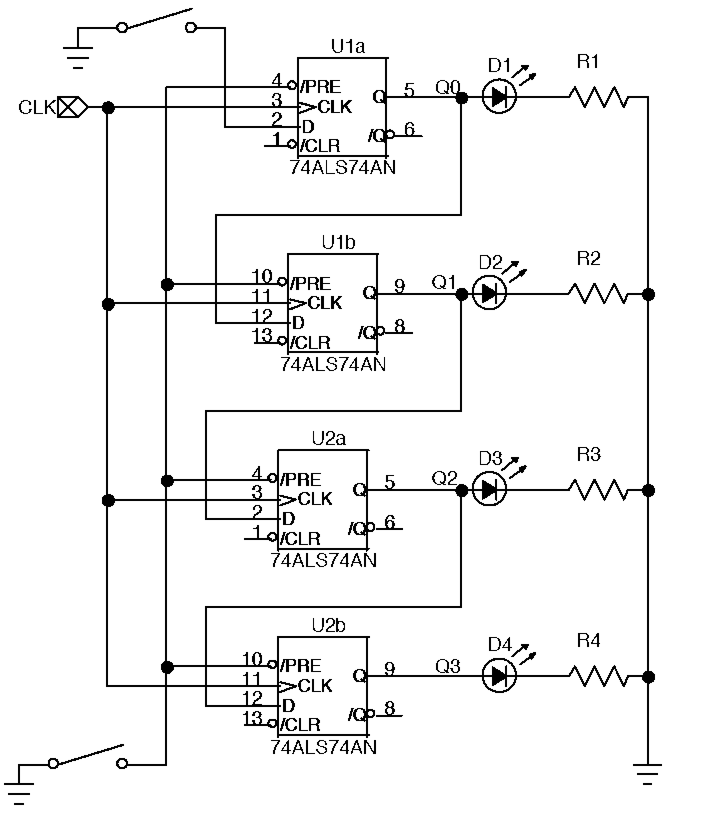
\includegraphics[scale=0.5]{shift.png}
		\caption{Schema dello shift register}
		\label{f:shift}
	\end{figure}

Gli ingressi CLR e PRE sono stati lasciati disconnessi senza osservare malfunzionamenti e rendendo quindi non necessarie le resistenze di pull-up.

Si è quindi proceduto ad inviare un clock a bassa frequenza (dell'ordine di $\sim\SI{1}{\hertz}$) per verificare il funzionamento del circuito: il bit inviato attraverso l'interruttore al primo D-Latch si propaga nei successivi ad ogni periodo di clock.
Lo stato delle uscite dopo aver premuto il pulsante di preset è HIGH, come atteso.
 
\section{Generatore di sequenze pseudo-casuali}
Si vuole realizzare un generatore di sequenze pseudo casuali a partire dallo shift register prima realizzato. Si sono collegati i due bit più significativi (Q2 e Q3, le uscite degli ultimi due D-Latch) ad una porta XOR, la cui uscita è stata collegata all'ingresso del primo D-Latch.
Si è quindi chiuso l'interruttore di preset e con un clock a bassa frequenza si è lasciato evolvere l'output.
Di seguito si riporta la sequenza osservata in un ciclo:

\begin{equation*}
\begin{matrix}
1)	&		&	1	&	1	&	1	&	1	\\
2)	&		&	0	&	1	&	1	&	1	\\
3)	&		&	0	&	0	&	1	&	1	\\
4)	&		&	0	&	0	&	0	&	1	\\
5)	&		&	1	&	0	&	0	&	0	\\
6)	&		&	0	&	1	&	0	&	0	\\
7)	&		&	0	&	0	&	1	&	0	\\
8)	&		&	1	&	0	&	0	&	1	\\
\end{matrix}
\qquad \qquad
\begin{matrix}
9)	&		&	1	&	1	&	0	&	0	\\
10)	&		&	0	&	1	&	1	&	0	\\
11)	&		&	1	&	0	&	1	&	1	\\
12)	&		&	0	&	1	&	0	&	1	\\
13)	&		&	1	&	0	&	1	&	0	\\
14)	&		&	1	&	1	&	0	&	1	\\
15)	&		&	1	&	1	&	1	&	0	\\
\end{matrix}
\end{equation*}